%%%%%%%%%%%%%%%%%%%%%%%%%%%%%%%%%%%%%%%%%%%%%%%%%%%
% DFJP Textbooks LaTeX Style Sample Document
% Version 1.0 (2020/01/09)
%
% Author:
% Petr Vnenk (petr.vnenk@upce.cz)
%
% Licence:
% Free for commercial use, no attribution required.
%
%%%%%%%%%%%%%%%%%%%%%%%%%%%%%%%%%%%%%%%%%%%%%%%%%%%

%-%-%-%-%-%-%-%-%-%-%-%-%-%-%-%-%-%-%-%-%-%-%-%
% 
% INTRODUCTORY SETTINGS AND PAGES
%
%-%-%-%-%-%-%-%-%-%-%-%-%-%-%-%-%-%-%-%-%-%-%-%

%------------------------------------------
% DEFINITION OF CLASS AND STYLE; "en_GB" set in first line for English grammar check (modify for grammar check in different language, e.g. cs_CZ for Czech)
%------------------------------------------

% !TeX spellcheck = en_GB
\documentclass[11pt,b5paper,twoside]{report}										% settings of font size, paper size and different margins on odd and even side
\usepackage{dfjp_vnenk}																% loads dfjp_vnenk.sty style file
\usepackage[
backend=biber															% !!! --->	% set biber instead of BibTex into compilator!
,style=iso-numeric
,sortlocale=en_GB														% !!! --->	% set local language environment ("cs_CZ" for Czech)!
,autolang=other
,bibencoding=UTF8
]{biblatex}																			% extended options of bibliography management
\addbibresource{bibliography.bib}										% !!! --->	% bibliography source file (modify according to your needs)

\begin{document}																	% beginning of document

\pagenumbering{arabic}																% type of page numbering

%------------------------------------------
% TITLE PAGE (vspace can be adjusted or replaced by vfill)
%------------------------------------------

\begin{center}
	\vspace*{2 cm}
	\renewcommand{\baselinestretch}{1.242}\selectfont								% vertical distance of rows in title
	\textbf{{\LARGE TITLE OF THE BOOK}}									% !!! --->	% add the title of the book here
	\thispagestyle{empty}															% removes page numbering from this page
	\renewcommand{\baselinestretch}{1}\selectfont									% vertical distance of rows returns to previous value after title
	
	\vspace{0.5 cm}
	Subtitle of the \textbf{Book}.
																		% !!! --->	% add the subtitle of the book here
	
	\vspace{1.5 cm}
	\textit{Petr Vnenk}													% !!! --->	% add the author of the book here
	
	\vspace{12 cm}
	University of Pardubice												% !!! --->	% add the publisher of the book here

	Pardubice 2020														% !!! --->	% add the town and year of publication of the book here
\end{center}

%------------------------------------------
% PAGE OF ACKNOWLEDGMENT AND IMPRINT
%------------------------------------------

\newpage																			% begins a new page
\textit{Lorem ipsum dolor sit amet, consectetur adipiscing elit, sed do eiusmod tempor incididunt ut labore et dolore magna aliqua. Ut enim ad minim veniam, quis nostrud exercitation ullamco laboris nisi ut aliquip ex ea commodo consequat.}

\textit{Duis aute irure dolor in reprehenderit in voluptate velit esse cillum dolore eu fugiat nulla pariatur. Excepteur sint occaecat cupidatat non proident, sunt in culpa qui officia deserunt mollit anim id est laborum.}

\textit{Sed ut perspiciatis unde omnis iste natus error sit voluptatem accusantium doloremque laudantium, totam rem aperiam, eaque ipsa quae ab illo inventore veritatis et quasi architecto beatae vitae dicta sunt explicabo.}		% !!! --->	% add the acknowledgement here

\vspace{10 cm}
VNENK, Petr. \textit{Title of the book.} Pardubice: University of Pardubice, 2020. 128~p. ISBN XXX-XX-XXXX-XXX-X.
																		% !!! --->	% add the "cite as" here

\vspace{2 cm}
Reviewed by: Name Surname, Name Surname									% !!! --->	% add the reviewers here

$ \copyright $ Ing.~Petr Vnenk, 2020									% !!! --->	% add the author and year of publication here

ISBN 978-80-7560-281-7													% !!! --->	% add the ISBN here
\thispagestyle{empty}																% removes page numbering from this page

%------------------------------------------
% TABLE OF CONTENTS
%------------------------------------------

\newpage																			% begins a new page
\begingroup
\tableofcontents																	% inserts table of contents
\addtocontents{toc}{\vspace{-30pt}}
\endgroup

%------------------------------------------
% LIST OF ABBREVIATIONS
%------------------------------------------

\newpage																			% begins a new page
\vspace*{1.32 cm}
\begin{fontoflistofabbreviations}													% inserts list of abbreviation (as a table)
	List of Abbreviations
\end{fontoflistofabbreviations}
\addcontentsline{toc}{chapter}{List of Abbreviations}
\vspace{1.65 cm}\\
\textit{in alphabetical order:}\\
\\
\begin{tabular}{ p{2cm} p{0.5cm} p{10.5cm} }
	ABB & -- & abbreviation\\ [1.242ex]
	ZKR & -- & \textit{Czech: zkratka}, abbreviation\\ [1.242ex]
\end{tabular}

%------------------------------------------
% LIST OF FIGURES
%------------------------------------------

\newpage																			% begins a new page
\listoffigures																		% inserts list of figures

%------------------------------------------
% LIST OF TABLES
%------------------------------------------

\newpage																			% begins a new page
\listoftables																		% inserts list of tables

%-%-%-%-%-%-%-%-%-%-%-%-%-%-%-%-%-%-%-%-%-%-%-%
% 
% BODY OF DOCUMENT
%
%-%-%-%-%-%-%-%-%-%-%-%-%-%-%-%-%-%-%-%-%-%-%-%

\chapter*{Introduction}
\addcontentsline{toc}{chapter}{Introduction}

This template was derived from the \textit{Základy stavebního práva} textbook published at the Faculty of Transport Engineering in 2020. You are free to use this template for any further works.

Some examples of the most common parts are presented after the next blank page.

Good luck in your work

\begin{flushright}
	\textit{Author}
\end{flushright}

\vspace{1 cm}
\textit{This template is updated by 24\textsuperscript{th}~February 2020.}

\afterpage{\null\newpage}												% !!! --->	% inserts a blank page (to start new chapter on odd page)

\chapter{First Level Heading}
\label{cha:flh}

This template generally contains three levels of headings -- chapters, sections and subsections. However, user is free to define others. The first level heading is here. It typically starts on an odd page.

\section{Second Level Heading}
\label{sec:slh}

This is the second level heading. Bibliography references can be attached as follows. \cite{enb1,osn1,kli1}

\subsection*{Third level Heading without Involvement in the Table of Content}
This is the third level heading. The asterisk means it won't show in the table of contents.

A quote can look like this:

\begin{displayquote}
	\textit{\uv{Art must not serve might.}}
	\begin{flushright}
		--- Karel Čapek~\cite{kli1}
	\end{flushright}
\end{displayquote}

\newpage
A table can look like this:

\begin{table}[h]
	
	\caption{This is a caption of the table below.}
	\begin{tabular}{ L{0.5\textwidth} C{0.2\textwidth} C{0.2\textwidth} }
		\textbf{Name} & \textbf{Year of Birth} & \textbf{Year of Death}\\
		\hline
		Tomáš Garrigue Masaryk & 1850 & 1937\\
		\specialrule{.05em}{0.1em}{0em}
		Tomáš Baťa & 1876 & 1932\\
		\specialrule{.05em}{0.1em}{0em}
		Karel Čapek & 1890 & 1938\\
		\hline
	\end{tabular}

\end{table}

And a figure can look like this:

\begin{figure}[h]
	
	\centering
	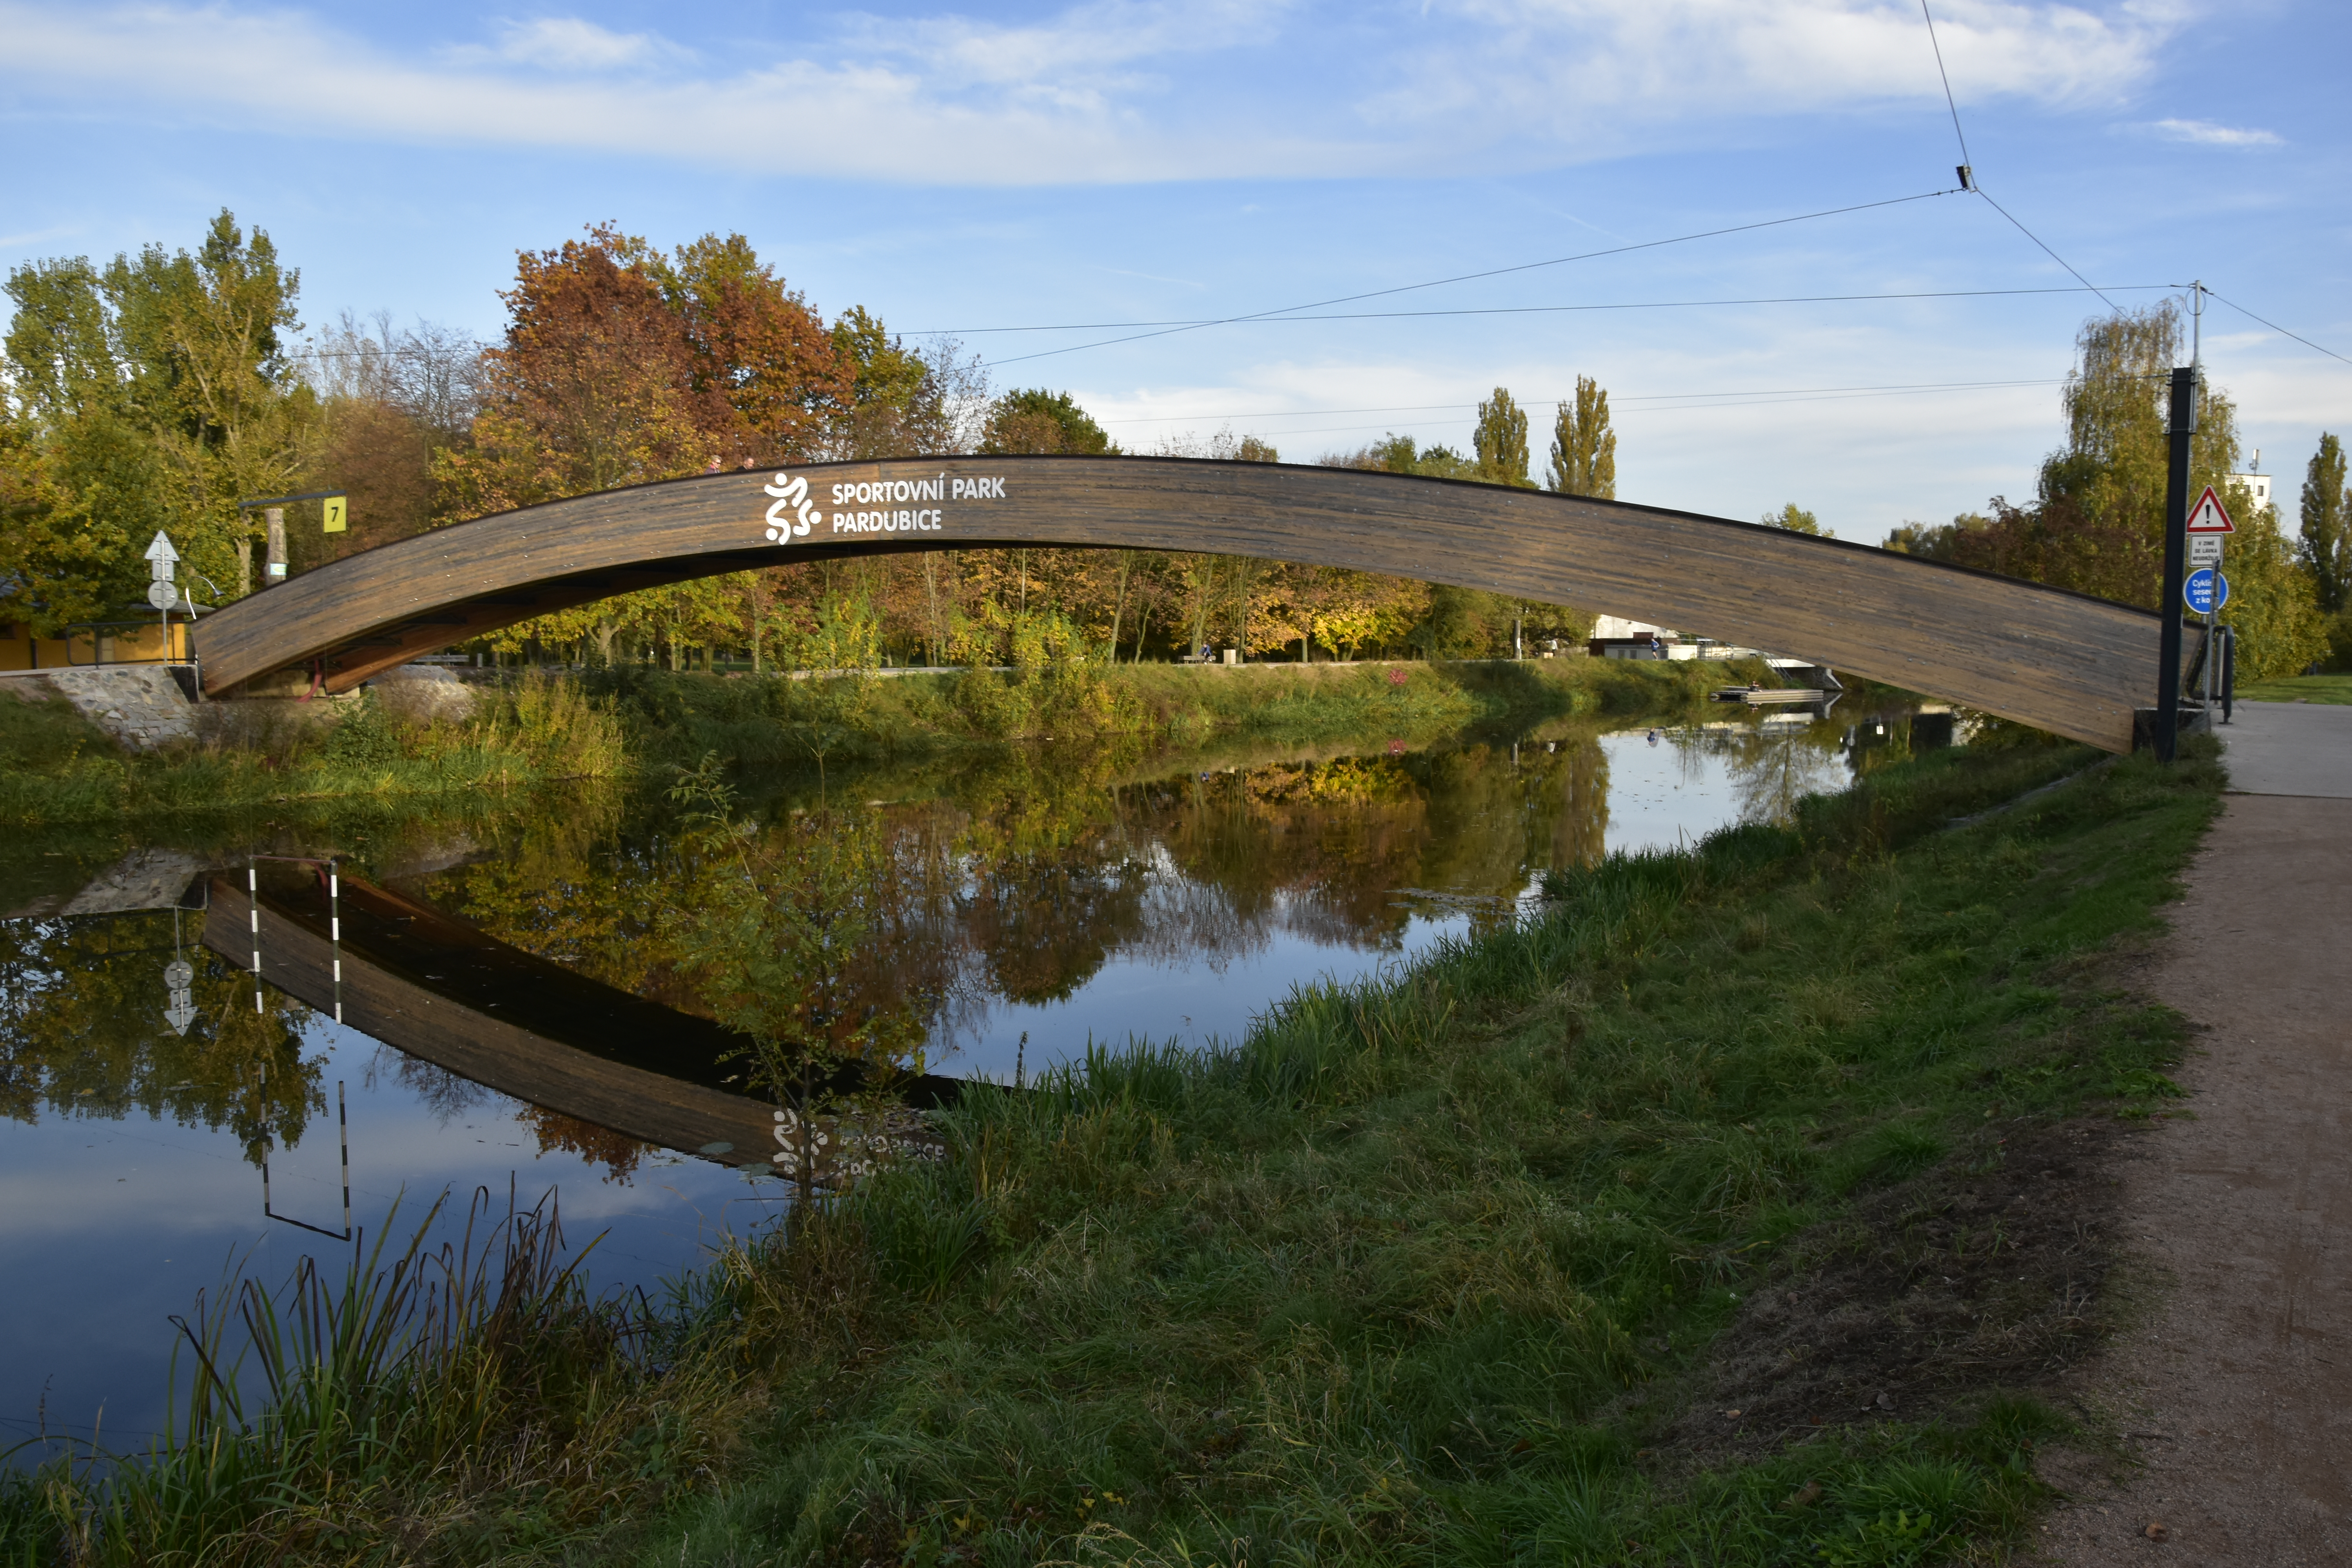
\includegraphics[width=1\textwidth]{na_spici}
	\caption{This is a caption of the figure above.}
	\label{fig:ns1}
	
\end{figure}

%-%-%-%-%-%-%-%-%-%-%-%-%-%-%-%-%-%-%-%-%-%-%-%
% 
% CLOSING SETTINGS AND PAGES
%
%-%-%-%-%-%-%-%-%-%-%-%-%-%-%-%-%-%-%-%-%-%-%-%

%------------------------------------------
% LIST OF BIBLIOGRAPHY
%------------------------------------------

\setcounter{biburllcpenalty}{7000}
\setcounter{biburlucpenalty}{8000}
\nocite{*}																			% includes bibliography, which is not cited in text, in the bibliography
\printbibliography[title={Bibliography},heading=bibintoc]							% prints out the list of bibliography

%------------------------------------------
% FINAL PAGE (including colophon)
%------------------------------------------

\newpage

\vspace*{14.5 cm}
\renewcommand{\baselinestretch}{1.242}\selectfont									% vertical distance of rows in title
\textbf{{\large TITLE OF THE BOOK}}										% !!! --->	% add the title of the book here
\thispagestyle{empty}																% removes page numbering from this page
\renewcommand{\baselinestretch}{1}\selectfont										% vertical distance of rows returns to previous value after title

Ing.~Petr Vnenk															% !!! --->	% add the author of the book here

\vspace{0.5 cm}
Published by University of Pardubice, Studentská~95, 532~10~Pardubice\newline
Printed by Polygrafic Center of the University of Pardubice\newline
Cover design by Name Surname\newline
1\textsuperscript{st} edition\newline
Pardubice~2020															% !!! --->	% add the colophon here
\vspace{0.5 cm}

ISBN XXX-XX-XXXX-XXX-X													% !!! --->	% add the ISBN here

\end{document}